\documentclass[tikz, border=10pt]{standalone}
\usepackage{tikz}
\usetikzlibrary{arrows.meta, shapes, positioning}
\usepackage{xcolor}
\definecolor{skyblue}{RGB}{135,206,235}
\tikzset{bigskybluenode/.style={circle, fill=skyblue, draw=black, line width=1pt},
smallskybluenode/.style={circle, fill=skyblue, draw=black, line width=0.5pt, minimum size=4pt, inner sep=0pt}}
\definecolor{cyan}{RGB}{0,255,255}
\tikzset{bigcyannode/.style={circle, fill=cyan, draw=black, line width=1pt},
smallcyannode/.style={circle, fill=cyan, draw=black, line width=0.5pt, minimum size=4pt, inner sep=0pt}}
\begin{document}
    % Graph for 3 attributes
    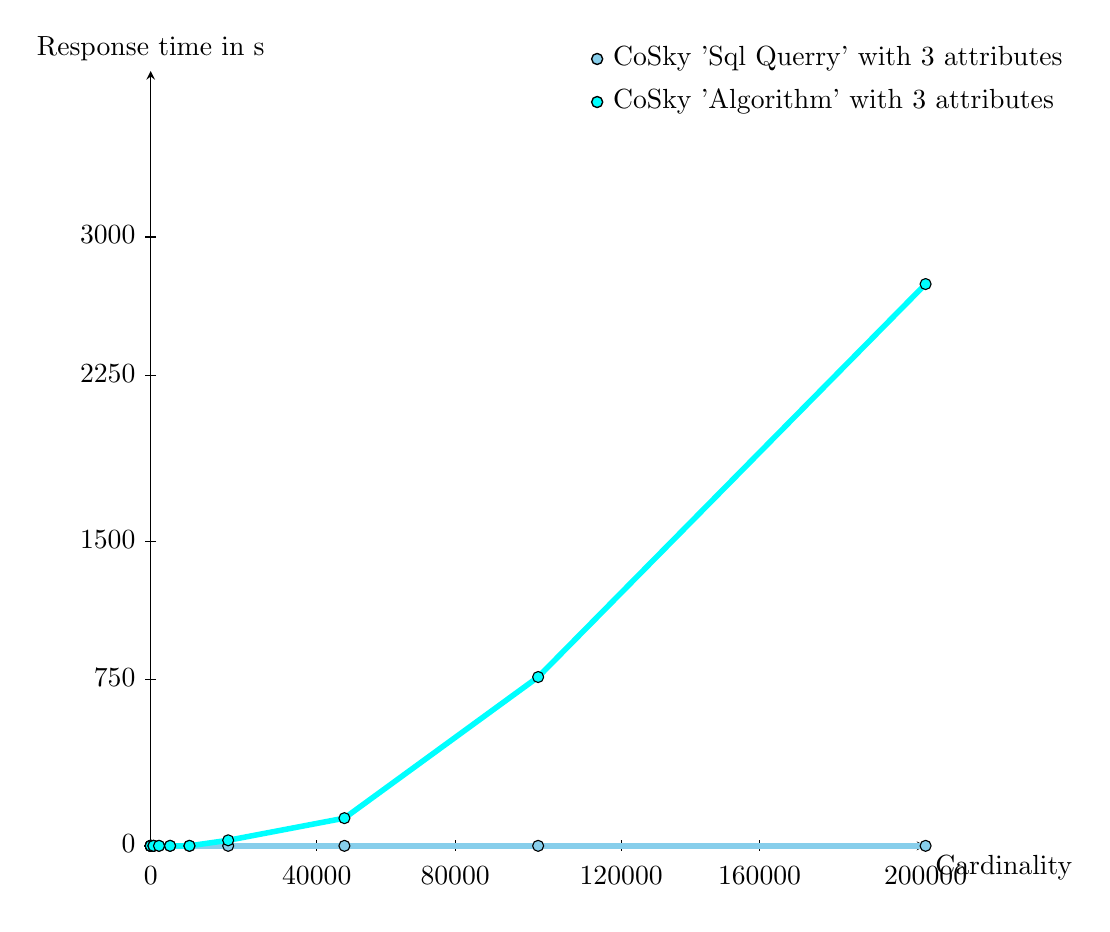
\begin{tikzpicture}[
        line join=bevel,
        bigskybluenode/.style={shape=circle, fill=skyblue, draw=black, line width=1pt},
        bigcyannode/.style={shape=circle, fill=cyan, draw=black, line width=1pt},
        smallskybluenode/.style={circle, fill=skyblue, draw=black, line width=0.5pt, minimum size=4pt, inner sep=0pt},
        smallcyannode/.style={circle, fill=cyan, draw=black, line width=0.5pt, minimum size=4pt, inner sep=0pt}
    ]
        % Axes
        \draw[-stealth] (0pt, 0pt) -- (280pt, 0pt) node[anchor=north west] {Cardinality};
        \draw[-stealth] (0pt, 0pt) -- (0pt, 280pt) node[anchor=south] {Response time in s};
        % Axis graduation
        \foreach \x/\xtext in {
            0pt/$0$, 
            60pt/$40000$, 
            110pt/$80000$, 
            170pt/$120000$, 
            220pt/$160000$, 
            280pt/$200000$} {
            \draw (\x, 2pt) -- (\x, -2pt) node[below] {\xtext\strut};
        }
        \foreach \y/\ytext in {
            0pt/$0$, 
            60pt/$750$, 
            110pt/$1500$, 
            170pt/$2250$, 
            220pt/$3000$} {
            \draw (2pt, \y) -- (-2pt, \y) node[left] {\ytext\strut};
        }
        % Lines
        \draw[skyblue, line width=2pt](0pt, 0pt) -- (0pt, 0pt) -- (0pt, 0pt) -- (0pt, 0pt) -- (0pt, 0pt) -- (1pt, 0pt) -- (1pt, 0pt) -- (3pt, 0pt) -- (7pt, 0pt) -- (14pt, 0pt) -- (28pt, 0pt) -- (70pt, 0pt) -- (140pt, 0pt) -- (280pt, 0pt);
        \draw[cyan, line width=2pt](0pt, 0pt) -- (0pt, 0pt) -- (0pt, 0pt) -- (0pt, 0pt) -- (0pt, 0pt) -- (1pt, 0pt) -- (1pt, 0pt) -- (3pt, 0pt) -- (7pt, 0pt) -- (14pt, 0pt) -- (28pt, 2pt) -- (70pt, 10pt) -- (140pt, 61pt) -- (280pt, 203pt);
        % Points
        \filldraw[color=black, fill=skyblue] (0pt, 0pt) circle (2pt);
        \filldraw[color=black, fill=skyblue] (0pt, 0pt) circle (2pt);
        \filldraw[color=black, fill=skyblue] (0pt, 0pt) circle (2pt);
        \filldraw[color=black, fill=skyblue] (0pt, 0pt) circle (2pt);
        \filldraw[color=black, fill=skyblue] (0pt, 0pt) circle (2pt);
        \filldraw[color=black, fill=skyblue] (1pt, 0pt) circle (2pt);
        \filldraw[color=black, fill=skyblue] (1pt, 0pt) circle (2pt);
        \filldraw[color=black, fill=skyblue] (3pt, 0pt) circle (2pt);
        \filldraw[color=black, fill=skyblue] (7pt, 0pt) circle (2pt);
        \filldraw[color=black, fill=skyblue] (14pt, 0pt) circle (2pt);
        \filldraw[color=black, fill=skyblue] (28pt, 0pt) circle (2pt);
        \filldraw[color=black, fill=skyblue] (70pt, 0pt) circle (2pt);
        \filldraw[color=black, fill=skyblue] (140pt, 0pt) circle (2pt);
        \filldraw[color=black, fill=skyblue] (280pt, 0pt) circle (2pt);
        \filldraw[color=black, fill=cyan] (0pt, 0pt) circle (2pt);
        \filldraw[color=black, fill=cyan] (0pt, 0pt) circle (2pt);
        \filldraw[color=black, fill=cyan] (0pt, 0pt) circle (2pt);
        \filldraw[color=black, fill=cyan] (0pt, 0pt) circle (2pt);
        \filldraw[color=black, fill=cyan] (0pt, 0pt) circle (2pt);
        \filldraw[color=black, fill=cyan] (1pt, 0pt) circle (2pt);
        \filldraw[color=black, fill=cyan] (1pt, 0pt) circle (2pt);
        \filldraw[color=black, fill=cyan] (3pt, 0pt) circle (2pt);
        \filldraw[color=black, fill=cyan] (7pt, 0pt) circle (2pt);
        \filldraw[color=black, fill=cyan] (14pt, 0pt) circle (2pt);
        \filldraw[color=black, fill=cyan] (28pt, 2pt) circle (2pt);
        \filldraw[color=black, fill=cyan] (70pt, 10pt) circle (2pt);
        \filldraw[color=black, fill=cyan] (140pt, 61pt) circle (2pt);
        \filldraw[color=black, fill=cyan] (280pt, 203pt) circle (2pt);
        % Caption
        \matrix [below left] at (current bounding box.north east) {
            \node [smallskybluenode, label=right:CoSky 'Sql Querry' with 3 attributes] {}; \\
            \node [smallcyannode, label=right:CoSky 'Algorithm' with 3 attributes] {}; \\
        };
    \end{tikzpicture}
    % Graph for 6 attributes
    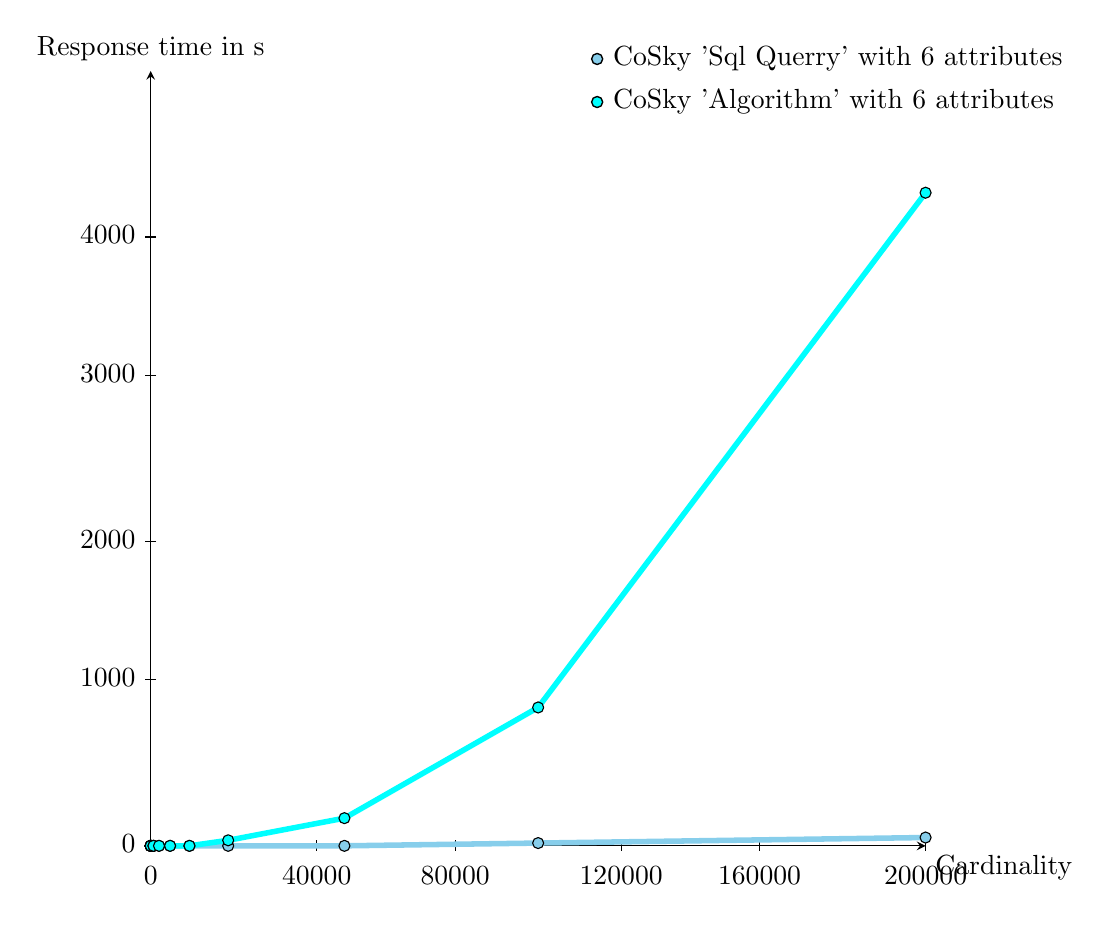
\begin{tikzpicture}[
        line join=bevel,
        bigskybluenode/.style={shape=circle, fill=skyblue, draw=black, line width=1pt},
        bigcyannode/.style={shape=circle, fill=cyan, draw=black, line width=1pt},
        smallskybluenode/.style={circle, fill=skyblue, draw=black, line width=0.5pt, minimum size=4pt, inner sep=0pt},
        smallcyannode/.style={circle, fill=cyan, draw=black, line width=0.5pt, minimum size=4pt, inner sep=0pt}
    ]
        % Axes
        \draw[-stealth] (0pt, 0pt) -- (280pt, 0pt) node[anchor=north west] {Cardinality};
        \draw[-stealth] (0pt, 0pt) -- (0pt, 280pt) node[anchor=south] {Response time in s};
        % Axis graduation
        \foreach \x/\xtext in {
            0pt/$0$, 
            60pt/$40000$, 
            110pt/$80000$, 
            170pt/$120000$, 
            220pt/$160000$, 
            280pt/$200000$} {
            \draw (\x, 2pt) -- (\x, -2pt) node[below] {\xtext\strut};
        }
        \foreach \y/\ytext in {
            0pt/$0$, 
            60pt/$1000$, 
            110pt/$2000$, 
            170pt/$3000$, 
            220pt/$4000$} {
            \draw (2pt, \y) -- (-2pt, \y) node[left] {\ytext\strut};
        }
        % Lines
        \draw[skyblue, line width=2pt](0pt, 0pt) -- (0pt, 0pt) -- (0pt, 0pt) -- (0pt, 0pt) -- (0pt, 0pt) -- (1pt, 0pt) -- (1pt, 0pt) -- (3pt, 0pt) -- (7pt, 0pt) -- (14pt, 0pt) -- (28pt, 0pt) -- (70pt, 0pt) -- (140pt, 1pt) -- (280pt, 3pt);
        \draw[cyan, line width=2pt](0pt, 0pt) -- (0pt, 0pt) -- (0pt, 0pt) -- (0pt, 0pt) -- (0pt, 0pt) -- (1pt, 0pt) -- (1pt, 0pt) -- (3pt, 0pt) -- (7pt, 0pt) -- (14pt, 0pt) -- (28pt, 2pt) -- (70pt, 10pt) -- (140pt, 50pt) -- (280pt, 236pt);
        % Points
        \filldraw[color=black, fill=skyblue] (0pt, 0pt) circle (2pt);
        \filldraw[color=black, fill=skyblue] (0pt, 0pt) circle (2pt);
        \filldraw[color=black, fill=skyblue] (0pt, 0pt) circle (2pt);
        \filldraw[color=black, fill=skyblue] (0pt, 0pt) circle (2pt);
        \filldraw[color=black, fill=skyblue] (0pt, 0pt) circle (2pt);
        \filldraw[color=black, fill=skyblue] (1pt, 0pt) circle (2pt);
        \filldraw[color=black, fill=skyblue] (1pt, 0pt) circle (2pt);
        \filldraw[color=black, fill=skyblue] (3pt, 0pt) circle (2pt);
        \filldraw[color=black, fill=skyblue] (7pt, 0pt) circle (2pt);
        \filldraw[color=black, fill=skyblue] (14pt, 0pt) circle (2pt);
        \filldraw[color=black, fill=skyblue] (28pt, 0pt) circle (2pt);
        \filldraw[color=black, fill=skyblue] (70pt, 0pt) circle (2pt);
        \filldraw[color=black, fill=skyblue] (140pt, 1pt) circle (2pt);
        \filldraw[color=black, fill=skyblue] (280pt, 3pt) circle (2pt);
        \filldraw[color=black, fill=cyan] (0pt, 0pt) circle (2pt);
        \filldraw[color=black, fill=cyan] (0pt, 0pt) circle (2pt);
        \filldraw[color=black, fill=cyan] (0pt, 0pt) circle (2pt);
        \filldraw[color=black, fill=cyan] (0pt, 0pt) circle (2pt);
        \filldraw[color=black, fill=cyan] (0pt, 0pt) circle (2pt);
        \filldraw[color=black, fill=cyan] (1pt, 0pt) circle (2pt);
        \filldraw[color=black, fill=cyan] (1pt, 0pt) circle (2pt);
        \filldraw[color=black, fill=cyan] (3pt, 0pt) circle (2pt);
        \filldraw[color=black, fill=cyan] (7pt, 0pt) circle (2pt);
        \filldraw[color=black, fill=cyan] (14pt, 0pt) circle (2pt);
        \filldraw[color=black, fill=cyan] (28pt, 2pt) circle (2pt);
        \filldraw[color=black, fill=cyan] (70pt, 10pt) circle (2pt);
        \filldraw[color=black, fill=cyan] (140pt, 50pt) circle (2pt);
        \filldraw[color=black, fill=cyan] (280pt, 236pt) circle (2pt);
        % Caption
        \matrix [below left] at (current bounding box.north east) {
            \node [smallskybluenode, label=right:CoSky 'Sql Querry' with 6 attributes] {}; \\
            \node [smallcyannode, label=right:CoSky 'Algorithm' with 6 attributes] {}; \\
        };
    \end{tikzpicture}
    % Graph for 9 attributes
    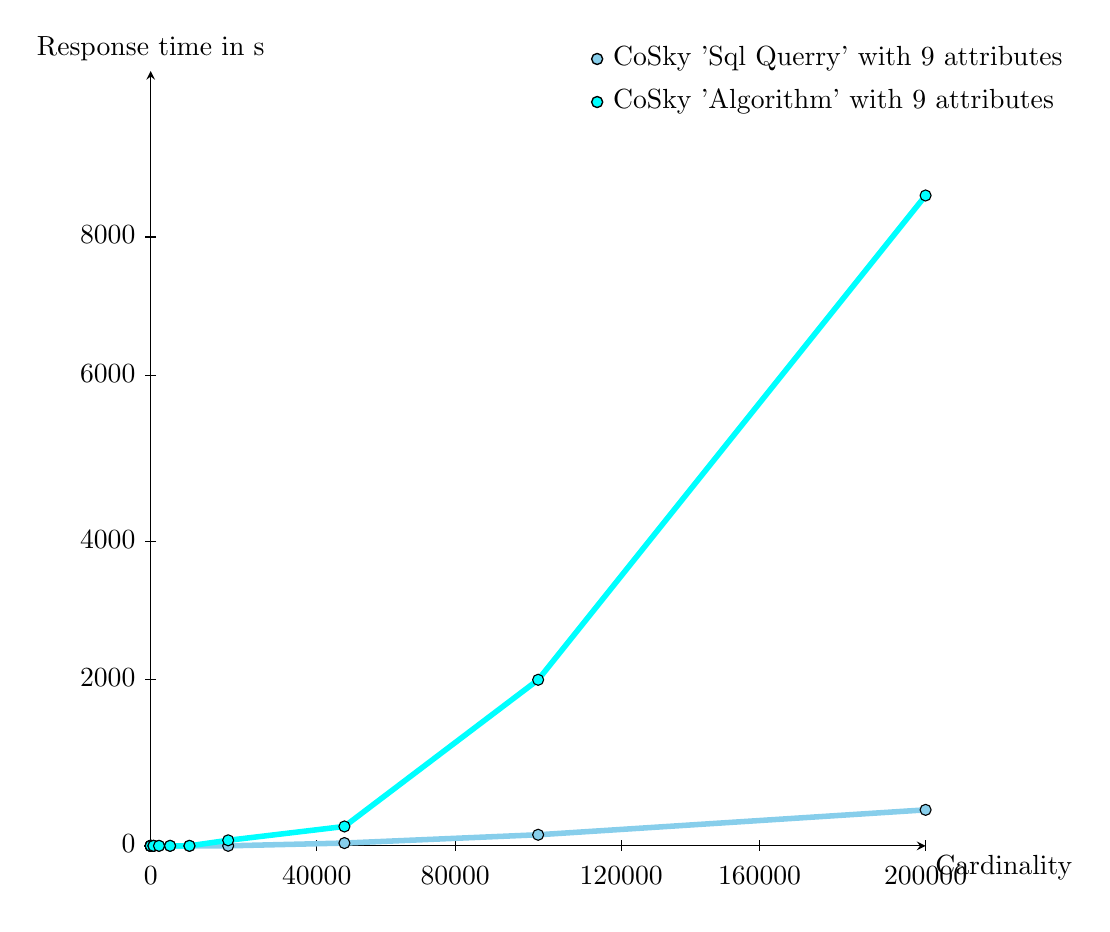
\begin{tikzpicture}[
        line join=bevel,
        bigskybluenode/.style={shape=circle, fill=skyblue, draw=black, line width=1pt},
        bigcyannode/.style={shape=circle, fill=cyan, draw=black, line width=1pt},
        smallskybluenode/.style={circle, fill=skyblue, draw=black, line width=0.5pt, minimum size=4pt, inner sep=0pt},
        smallcyannode/.style={circle, fill=cyan, draw=black, line width=0.5pt, minimum size=4pt, inner sep=0pt}
    ]
        % Axes
        \draw[-stealth] (0pt, 0pt) -- (280pt, 0pt) node[anchor=north west] {Cardinality};
        \draw[-stealth] (0pt, 0pt) -- (0pt, 280pt) node[anchor=south] {Response time in s};
        % Axis graduation
        \foreach \x/\xtext in {
            0pt/$0$, 
            60pt/$40000$, 
            110pt/$80000$, 
            170pt/$120000$, 
            220pt/$160000$, 
            280pt/$200000$} {
            \draw (\x, 2pt) -- (\x, -2pt) node[below] {\xtext\strut};
        }
        \foreach \y/\ytext in {
            0pt/$0$, 
            60pt/$2000$, 
            110pt/$4000$, 
            170pt/$6000$, 
            220pt/$8000$} {
            \draw (2pt, \y) -- (-2pt, \y) node[left] {\ytext\strut};
        }
        % Lines
        \draw[skyblue, line width=2pt](0pt, 0pt) -- (0pt, 0pt) -- (0pt, 0pt) -- (0pt, 0pt) -- (0pt, 0pt) -- (1pt, 0pt) -- (1pt, 0pt) -- (3pt, 0pt) -- (7pt, 0pt) -- (14pt, 0pt) -- (28pt, 0pt) -- (70pt, 1pt) -- (140pt, 4pt) -- (280pt, 13pt);
        \draw[cyan, line width=2pt](0pt, 0pt) -- (0pt, 0pt) -- (0pt, 0pt) -- (0pt, 0pt) -- (0pt, 0pt) -- (1pt, 0pt) -- (1pt, 0pt) -- (3pt, 0pt) -- (7pt, 0pt) -- (14pt, 0pt) -- (28pt, 2pt) -- (70pt, 7pt) -- (140pt, 60pt) -- (280pt, 235pt);
        % Points
        \filldraw[color=black, fill=skyblue] (0pt, 0pt) circle (2pt);
        \filldraw[color=black, fill=skyblue] (0pt, 0pt) circle (2pt);
        \filldraw[color=black, fill=skyblue] (0pt, 0pt) circle (2pt);
        \filldraw[color=black, fill=skyblue] (0pt, 0pt) circle (2pt);
        \filldraw[color=black, fill=skyblue] (0pt, 0pt) circle (2pt);
        \filldraw[color=black, fill=skyblue] (1pt, 0pt) circle (2pt);
        \filldraw[color=black, fill=skyblue] (1pt, 0pt) circle (2pt);
        \filldraw[color=black, fill=skyblue] (3pt, 0pt) circle (2pt);
        \filldraw[color=black, fill=skyblue] (7pt, 0pt) circle (2pt);
        \filldraw[color=black, fill=skyblue] (14pt, 0pt) circle (2pt);
        \filldraw[color=black, fill=skyblue] (28pt, 0pt) circle (2pt);
        \filldraw[color=black, fill=skyblue] (70pt, 1pt) circle (2pt);
        \filldraw[color=black, fill=skyblue] (140pt, 4pt) circle (2pt);
        \filldraw[color=black, fill=skyblue] (280pt, 13pt) circle (2pt);
        \filldraw[color=black, fill=cyan] (0pt, 0pt) circle (2pt);
        \filldraw[color=black, fill=cyan] (0pt, 0pt) circle (2pt);
        \filldraw[color=black, fill=cyan] (0pt, 0pt) circle (2pt);
        \filldraw[color=black, fill=cyan] (0pt, 0pt) circle (2pt);
        \filldraw[color=black, fill=cyan] (0pt, 0pt) circle (2pt);
        \filldraw[color=black, fill=cyan] (1pt, 0pt) circle (2pt);
        \filldraw[color=black, fill=cyan] (1pt, 0pt) circle (2pt);
        \filldraw[color=black, fill=cyan] (3pt, 0pt) circle (2pt);
        \filldraw[color=black, fill=cyan] (7pt, 0pt) circle (2pt);
        \filldraw[color=black, fill=cyan] (14pt, 0pt) circle (2pt);
        \filldraw[color=black, fill=cyan] (28pt, 2pt) circle (2pt);
        \filldraw[color=black, fill=cyan] (70pt, 7pt) circle (2pt);
        \filldraw[color=black, fill=cyan] (140pt, 60pt) circle (2pt);
        \filldraw[color=black, fill=cyan] (280pt, 235pt) circle (2pt);
        % Caption
        \matrix [below left] at (current bounding box.north east) {
            \node [smallskybluenode, label=right:CoSky 'Sql Querry' with 9 attributes] {}; \\
            \node [smallcyannode, label=right:CoSky 'Algorithm' with 9 attributes] {}; \\
        };
    \end{tikzpicture}
\end{document}